\documentclass[11pt, oneside]{book}

\usepackage{geometry}[letterpaper]
\usepackage{amsmath, amssymb, amsthm}

\newcommand{\R}{\mathbb{R}}
\usepackage{graphicx}

\begin{document}

\chapter{Weeks 1}

ECEN-689
Dr. Zhiwen Fan
TTh 9:35 AM - 10:50 AM
AIEN M113

\section{Introduction -- 1/13}

Geometry, semantics, affordance, actionable information

\section{Introduction \& Guest Lectuer - 1/15}

Hezhen Hu
performance drops for users and contexts in the long tail
inclusion: how to build models that generalize to diverse humans across bodies, context
core: human foundational models
embodiment -> inclusive; understanding -> context-aware
general visual benchmark million=level (datacomp, panda)
human-centric datasets: thousand-level (CSL-daily-21k; dymvhuman)
training human foundation model (web data - vast scale, low quality)
BERT success in MLP; can this pretraining strategy work for human video

words: rich semantics, discrete, high-level
video: low info densit, continuous, redundant

three key components: visual token; pretraing strat; human prior
visual token: compact human pose (input -> visual token -> GCN -> input embedding)
filters irrelevant information
reduces redundancy (reduce input dimension by 2,000+ times)
multi-level masking (randomly mask joints; randomly mask frames; randomly mask frames)
prelim: MANO: parametric hand model
MANO is pre-learned from large hand scans (provide mapping)
MPL -> MANO ()\& proj) -> projection -> hand reconstruction
SignBERT shows versatile capability on multiple sign language understanding tasks

EVA: expressive human modeling from in-the-wild video
\#1 expressive animatable avatar
\#2 simple rbg video input (no human mesh annotation required)

monocular rgb video -> smpl-x alignment -> gaussian avatar modeling -> animate avatar
multi esimators: 2d pose (dwpose) \& 3d body (smpler-x) \& 3d hand (hamer)
all goes to iterative fitting to extract each models complimentary strengths

HumanNOVA: efficient avatar modeling from a single image
data: scalable data generation pipeline
model: scalable transformer backbone

data: synthetic data generation (rigged human mesh -> (smpl-x pose) -> animated mesh \& render)
real-world data generation (multi-view captured data -> (3dgs fitting) -> 3dgs assets \& render)

model: multi-modal encoding; incorporate human coarse mesh as human prior
2d-to-3d mapping: triplane as 3d representation; updated from multi-modal encoding via cross-attn

MMHU: scalable data annomation pipeline
* large-scale video collection (paid/collected; YouTube video; Waymo video)
* into low-level context (pose \& description) goes into
* high-level semantics (behavior \& intent)

Future:
* human-centric 3d foundation model: current foundation model only sees people;
desired model understands people in 3d and context
1. scalable data infrastructure -> human-centric 3d foundation model -> diverse downstream tasks
2. human-centric 3d foundation model (unified model): structured human encoder -> unified latent space (geo, contact, motion, context, intent)
3. 3d human understanding \& gen, interaction \& intent prediction, ...

* embodied active reasoning (from passive perception to active human understanding)
passive vision model (static camera) leads to unsafe action
active agent (dynamic interactives) leads to SAFE action
observe, reason: belief-aware human state representation -> active reasoning

* embodied social affordance learning: enable agents to support effective and inclusive multi-person collaboration
agent needs to understand role of each person and their reactions
read social cues in (understanding) -> reason \& react with social knowledge (reason) -> output predictions in more socially-suitable way!

---------------------

main lecture:

current state of the art: many less than 5 years
* cv still active research area, rapidly changing
* deep learning and generative methods powering many modern applications

why is cv difficult $\rightarrow$ viewpoint variation, illumination, scale
* also intra-class vision (concepts), motion, background clutter, occlusion
* perception is an inherently ambiguous problem; must often use prior knowledge about the world's structure

\pagebreak

\section{Week 2 -- Jan 22}

\section{Week 2 -- Jan 22}

% student one
\subsection{Student 1}
\subsubsection{BEVFormer}
In autonomous driving, car needs to understand the whole scene around it, using cameras that each see only part of the world.

Need a unified, ego-centric representation that puts everything into one shared view.

BEV Queries, grid where we want to know what is present.

BEV architecture: two key architectures: spatial cross-attention and temporal self-attention.

Sparse cross attention: full BEV-to-image cross-attention is too expensive. BEVFormer proposes sparse spatial cross-attention. Each BEV query efficient uses most relevant camera.

Temporal self-attention: fuses history in a recurrent way, since pure memory would be too costly

BEVFormer builds a unified BEV representation from multi-camera images with a query-based transformer. Directly contructs BEV.

\subsubsection{VoxFormer}
Model needs to predict voxel grid in 3D space. If object is identified, needs to predict semantic class. Model infers in visible surface and occluded space as well so 3D volume is complete, model has to reason occluded geometry. \\

Compared to BEV-based detection. Natively apply BEV feature, still much heavier, use sparse voxel representation. Use important elements of query proposals to reduce computational cost. Result is improved performance over MonoScene since only relevant query proposals is sent to transformer, helps model focus on important 3D locations. \\

2D features are extracted by ResNet50 from RGB images, amd depth is estimated by depth predictor. \\

VoxFormer targets camera-based 3D semantics scene completion and makes 3D reasoning feasible via sparse voxle tokens. Key design: depth/occupancy-guided query proposal + deformable attention, then mask-token completion in voxel space.

% student two
\subsection{Student 2 -- Dayou Li -- Latent Action}

Bottleneck in robot learning: large-scale robot datasets are expensive to collect, require robot hardware, but contain robot action. Internet-scale video data is widely available, but there is a human to robot gap, and no included robot information.

\subsubsection{LAPA -- Latent action pretraining from video}
Latent action quantization: change in current to observation to predict latent action (VLM) LAPA determines action. 1. latent action quantization. 2. latent pretraining 3. LAPA $\rightarrow$ action.

Latent action encoding: input of current and next frame, patch embed, spatial transformer, causal transformer which outputs transition of two embeddings.
\[
    z_1 = \arg \min_{z_k} |d_1 - z_k|^2
\]
\[
    L = ||x_2 - \hat{x}_2||^2
\]
This model is compared to OpenVLA, ActionVLA, outperformed them. \\

Reconstruction loss is supervisation. Want latent actions to predict.

\subsubsection{CLAP model}
Supervised in both reconstruction in visualization and action space. \\

Pipeline: Act-VAE action trajector $\rightarrow$ codebook $\rightarrow$ decode action \\

VD-VAE: visual feature of the current frame and another frame, encoded by Dyno (can use another pretraining encoder), outputs two branches $z_{q, a}$ and $z_{q, i}$, these two branches go to encoder with first frame and outputs last frame as the supervisation. \\

CLAP-NTP: VLM to turn obs and instr to subtack and action tokens \\

CLAP-RF: uses VLM backbones that encode current vision and language context \\

Conclusions: latent actions provide a scalable token interface for learning from videos, which is valuable for cross-embodiment learning. LAPA shows that video-only tokenization can work and can leverage human videos, but tokens many be visually entangled and require action finetuning for executability. CLAP strengthens grounding by aligning video latents to robot actions latents and adds a planner-controller style.



\section{Week 3 -- Jan 27}
Text-to-image generation; DALL-E 2;

Textual token: turn input text into tokens, encoder needs to be fully well-trained with web-scale data. CLIP objective is the go between to the image encoder.

DALL-E 3;

GPT-4;

Segment Anything Model (SAM), large image model, very high-scale segmentation.

\subsection{Neural networks -- the original linear classifier}
(Before) Linear score function: $f = Wx$.
(Now): 2-layer neural network: $f = W_2 \max(0, W_1 x)$.
where $x \in \R^D$, $W_1 \in \R^{H \times D}$, $W_2 \in \R^{C \times H}$.

ReLU still used commonly as activation function, good default choice for most problems.
Leaky ReLU has small weight on left side. \\

Forward processing is done at inference time. Backward processing is done at training time. \\

\subsubsection{Computing gradients}
$ s = f(x; W_1, W_2) = W_2 \max(0, W_1 x) $ nonlinear score function; \\

$ L_i = \sum_{j \neq y_i} \max(0, s_j - s_{y_i} + 1) $ hinge loss on predictions; \\

$ R(W) = \sum_{k} W_k ^2 $ regularization; \\

$ L = \frac{1}{N} \sum_i L_i + \lambda R(W) $ total loss: data loss + regularization

\subsubsection{Backpropagation in Neutral Networks}
$ f(x, y, z) = (x + y)z $ \\
$ q = x + y $ \\
$ f = qz $ \\
Then, by chain rule,
\[
    \frac{\partial f}{\partial x} = \frac{\partial f}{\partial q} \frac{\partial q}{\partial x} = z \cdot 1 = z
\]
\[
    \frac{\partial f}{\partial y} = \frac{\partial f}{\partial q} \frac{\partial q}{\partial y} = z \cdot 1 = z
\]
\[    \frac{\partial f}{\partial z} = \frac{\partial f}{\partial q} \frac{\partial q}{\partial z} = q \cdot 1 = x + y
\]

\subsubsection{Regularization intuition: prefer simpler models}

\begin{figure}[hbpt!]
    \centering
    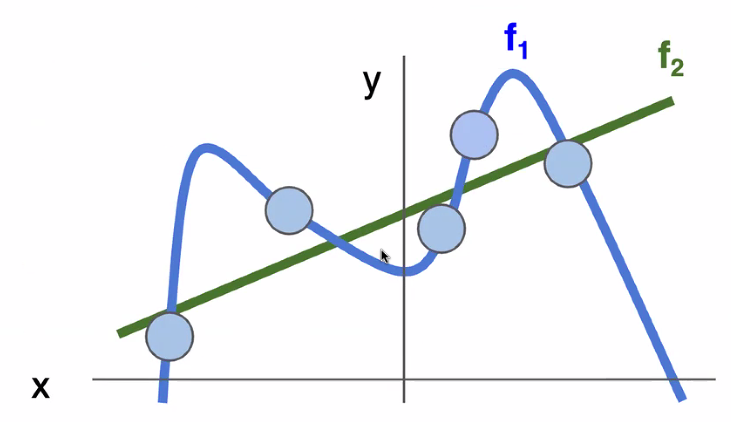
\includegraphics[width=0.5\textwidth]{figures/regularization1.png}
    \caption{Regularization prefers simpler models that generalize better.}
\end{figure}

When the model starts to overfit, training accuracy rises, but validation accuracy drops.

\begin{figure}[hbpt!]
    \centering
    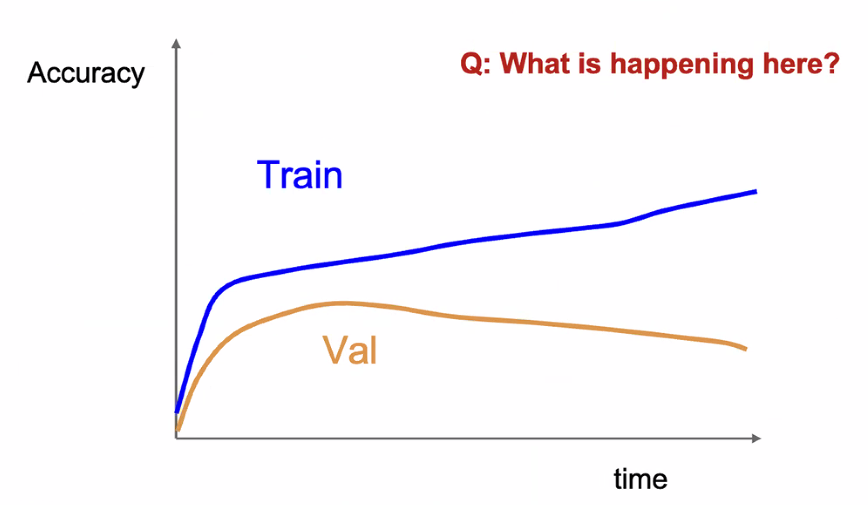
\includegraphics[width=0.5\textwidth]{figures/regularization2.png}
    \caption{Regularization prefers simpler models that generalize better.}
\end{figure}

Regularization:
\[
    L(W) = \frac{1}{N} \sum_i \underbrace{L_i(f(x_i, W), y_i)}{data loss: model predictions should match training data} + \underset{regularization: prevent the model from doing too well on training data}{\lambda R(W)}
\]

\subsubsection{Components of CNNs}
convolutional layers: normalization layers $\hat{x}_{i, j} = \frac{x_{i, j} - \mu_{j}}{\sqrt{\sigma_j^2 + \epsilon}}$;

pooling layers; dropout (sometimes); fully-connected layers; activation functions (ReLU, sigmoid, tanh, softmax).


\end{document}